% Created 2021-02-08 lun 10:23
% Intended LaTeX compiler: pdflatex
\documentclass[presentation,aspectratio=169]{beamer}
\usepackage[utf8]{inputenc}
\usepackage[T1]{fontenc}
\usepackage{graphicx}
\usepackage{grffile}
\usepackage{longtable}
\usepackage{wrapfig}
\usepackage{rotating}
\usepackage[normalem]{ulem}
\usepackage{amsmath}
\usepackage{textcomp}
\usepackage{amssymb}
\usepackage{capt-of}
\usepackage{hyperref}
\usepackage{khpreamble}
\usepackage{amssymb}
\usepgfplotslibrary{groupplots}
\newcommand*{\shift}{\operatorname{q}}
\usetheme{default}
\author{Kjartan Halvorsen}
\date{2021-02-08}
\title{Análisis de elementos de la mecatrónica}
\hypersetup{
 pdfauthor={Kjartan Halvorsen},
 pdftitle={Análisis de elementos de la mecatrónica},
 pdfkeywords={},
 pdfsubject={},
 pdfcreator={Emacs 26.3 (Org mode 9.4.4)}, 
 pdflang={English}}
\begin{document}

\maketitle

\section{Presentación}
\label{sec:org63c16a5}
\begin{frame}[label={sec:orgcaf0661}]{¿Quién soy yo}
\begin{center}
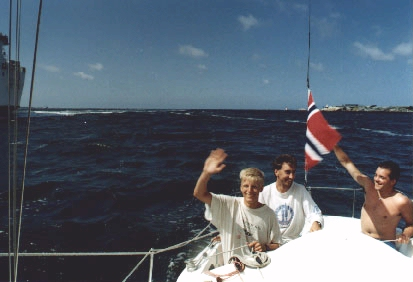
\includegraphics[height=0.6\textheight]{../../figures/red-heat-2.jpeg}
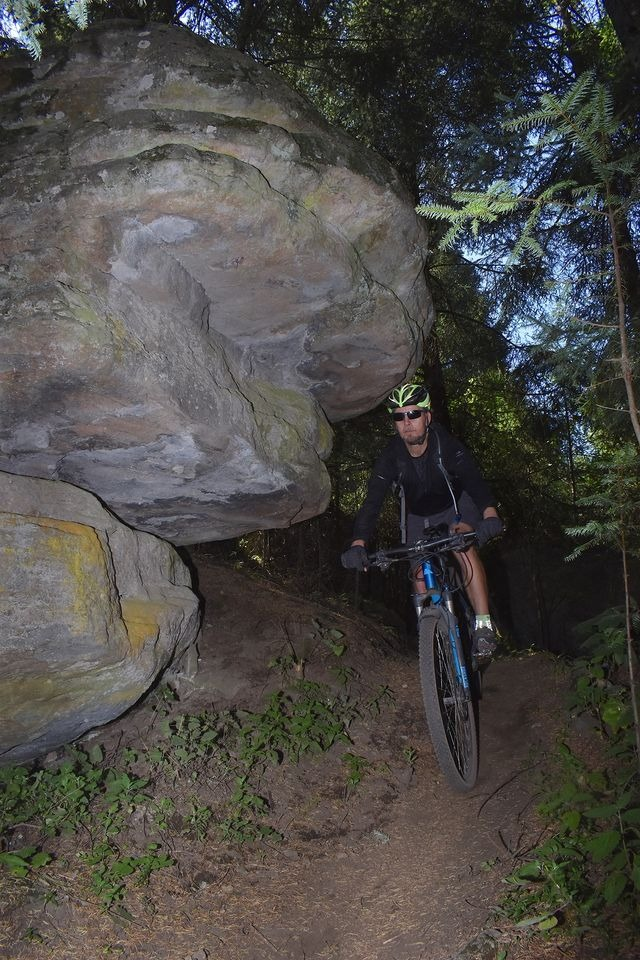
\includegraphics[height=0.6\textheight]{../../figures/mtb.jpeg}
\end{center}
\end{frame}




\begin{frame}[label={sec:orgdcd4c66}]{¿Quién eres tú?}
\end{frame}


\section{Intro}
\label{sec:org5e393b7}
\begin{frame}[label={sec:orgc57501e}]{Objetivos, contenido, evaluación}
\end{frame}


\section{Sistemas mecatrónicos}
\label{sec:orgf14e70c}

\begin{frame}[label={sec:orgb79af90}]{Sistemas mecatrónicos}
\end{frame}

\begin{frame}[label={sec:org7ff5547}]{Eso \alert{no} es un yate \alert{ni} un sistema mecatrónico}
\begin{center}
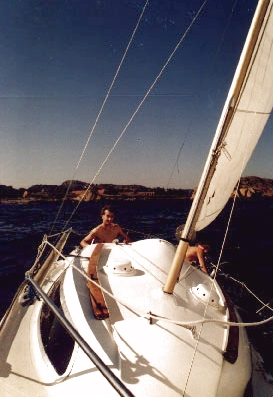
\includegraphics[height=0.6\textheight]{../../figures/red-heat-1.jpeg}
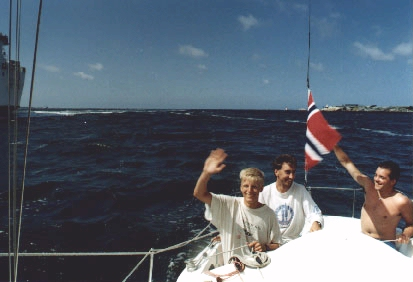
\includegraphics[height=0.6\textheight]{../../figures/red-heat-2.jpeg}
\end{center}
\end{frame}

\begin{frame}[label={sec:org16f6c9b}]{Eso \alert{sí} es un yate \alert{y} un sistema mecatrónico}
\begin{center}
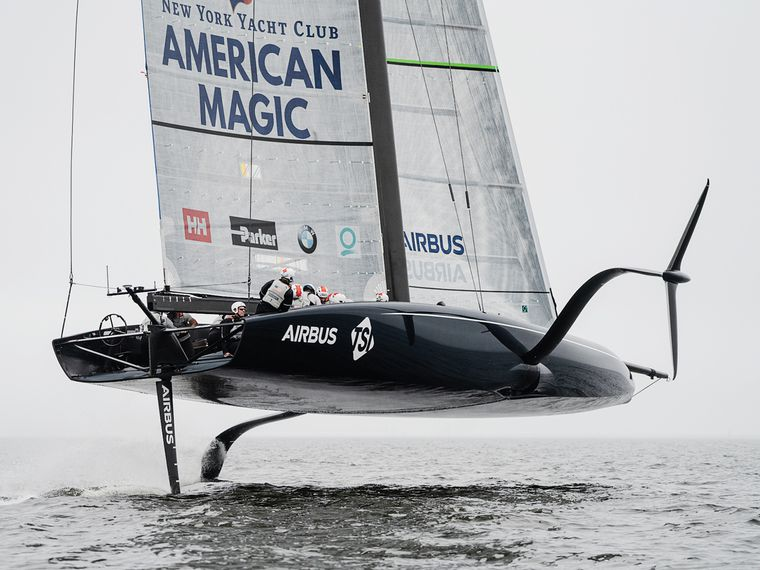
\includegraphics[height=0.7\textheight]{../../figures/ac75.jpeg}\\
{\footnotesize  From SailingWorld}
\end{center}

\href{https://www.sailingscuttlebutt.com/wp-content/uploads/2018/03/AC75\_Class\_Rule.pdf}{AC75 Class rule}
\end{frame}

\begin{frame}[label={sec:org9c5253c}]{Videos}
\url{https://youtu.be/VQUl\_hf6yo8}

\url{https://youtu.be/pDn3JVnw\_EI}

\url{https://youtu.be/\_B37zmJpBv4}
\end{frame}

\begin{frame}[label={sec:org541757c}]{Análisis del sistema}
\begin{block}{Requisitos o criterios de diseño}
\end{block}

\begin{block}{Identificar y describir elementos del sistem}
\begin{itemize}
\item Mecanismo
\item Actuadores
\item Sensores
\item Sistema de control
\end{itemize}
\end{block}
\end{frame}

\begin{frame}[label={sec:org9fd4645}]{Requisitos o criterios de diseño}
 \begin{center}
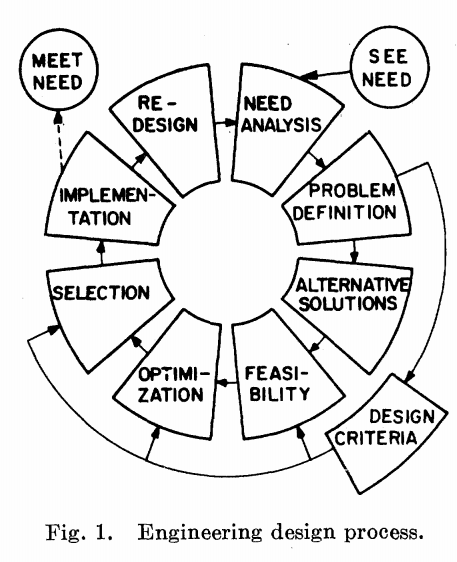
\includegraphics[height=0.6\textheight]{../../figures/design-process-fig1.png}\\
{\footnotesize  S.F. Love (1969) Modern design methods for electronics IEEE Tr Systems Science and Cybernetics}
\end{center}
\end{frame}

\begin{frame}[label={sec:org4e6f287}]{Sistema de hidroalas}
 \begin{center}
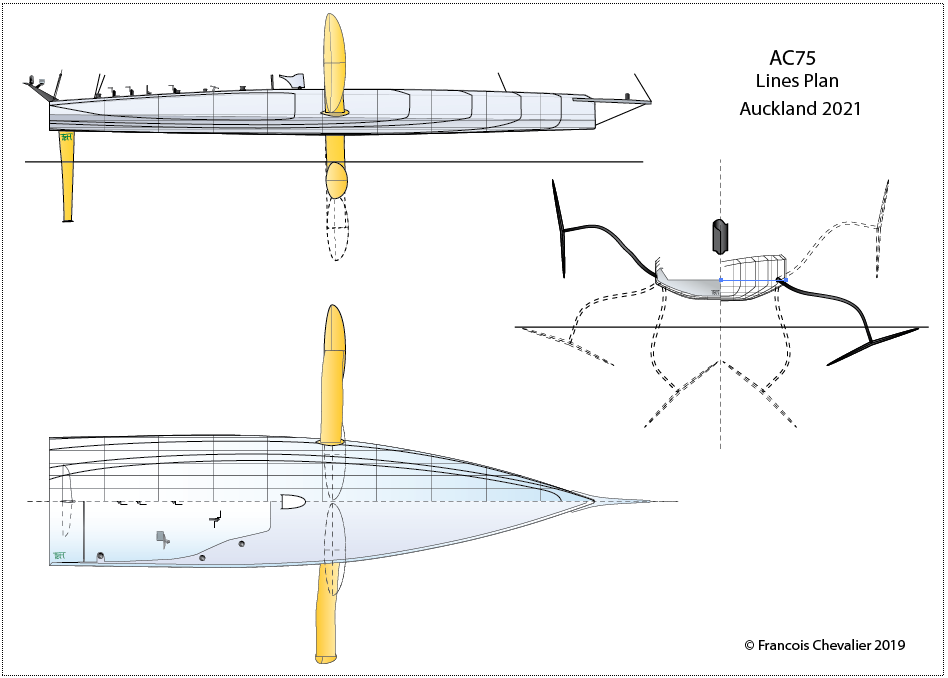
\includegraphics[height=0.6\textheight]{../../figures/AC75-lines.png}
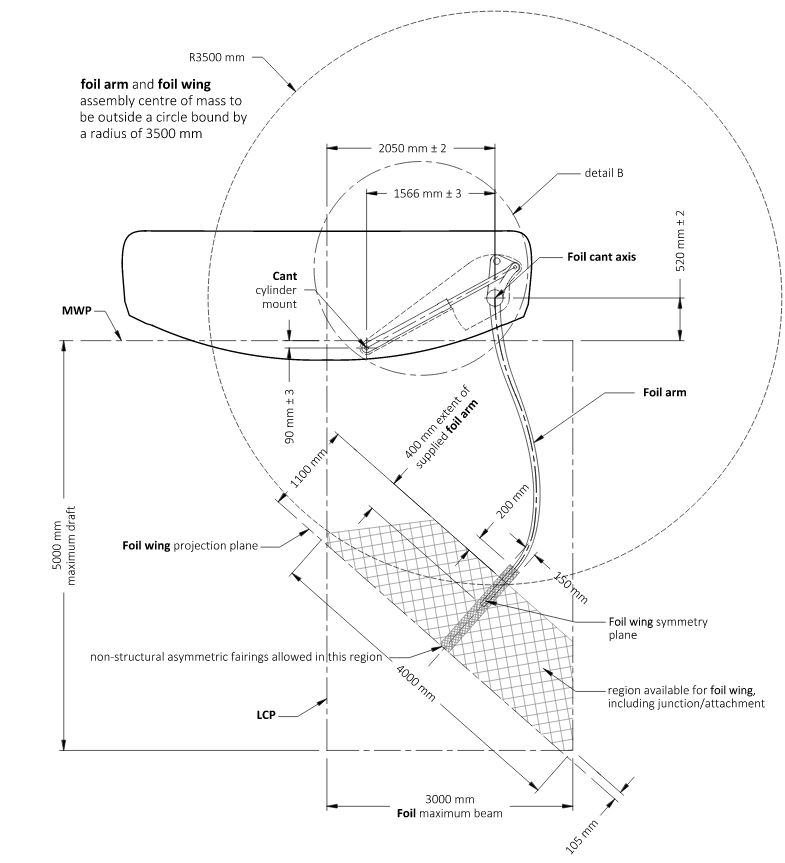
\includegraphics[height=0.7\textheight]{../../figures/AC75-class-foil.png}\\
{\footnotesize  By François Chevalier \hfill From the AC75 Class Rule}
\end{center}
\end{frame}


\begin{frame}[label={sec:org40cbbe9}]{Sistema de hidroalas}
\begin{columns}
\begin{column}{0.5\columnwidth}
\begin{center}
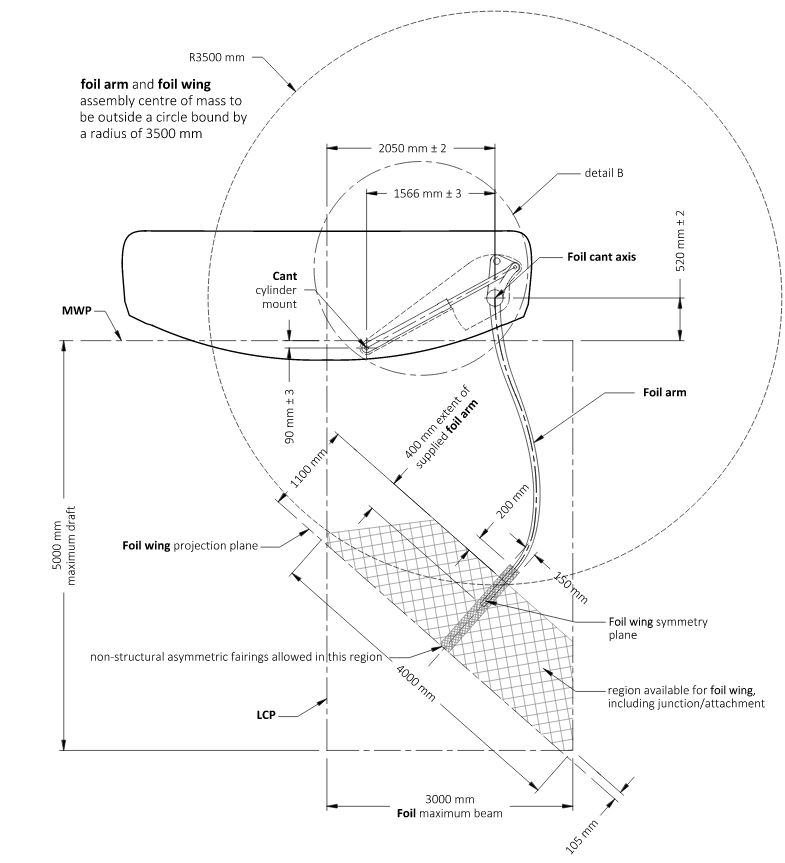
\includegraphics[height=0.8\textheight]{../../figures/AC75-class-foil.png}
\end{center}

{\footnotesize From the AC75 Class Rule}
\end{column}
\begin{column}{0.5\columnwidth}
\begin{itemize}
\item Displacamiento (masa total) - 7.6 t
\item Masa de cada ala - 1.2 t
\item Altura del mástil - 28m
\item Área de vela - 235 sqm
\item Profundidad máxima con alas - 5m
\end{itemize}
\end{column}
\end{columns}
\end{frame}

\begin{frame}[label={sec:orga72b923}]{Sistema de hidroalas - Requisitos}
\begin{center}
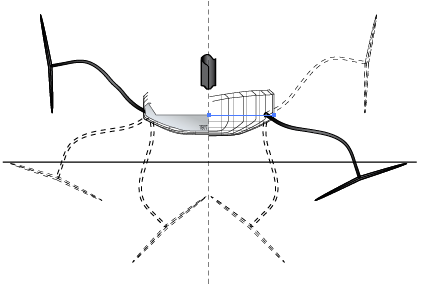
\includegraphics[height=0.2\textheight]{../../figures/AC75-sketch.png}
{\footnotesize  By François Chevalier}
\end{center}

El sistema debe
\begin{itemize}
\item Por medio del flujo de agua sobre al ala producir suficente fuerza para levantar el yate.
\item Sústener fuerzas hasta 1000 kN en el ala en posición fija.
\item Poder cambiar la dirección de la dicha fuerza.
\item Poder cambiar la posición del ala para funcionar como ala o como contrapeso.
\item Poder mover la posición de la ala en un rango de 50 grados en menos de 3 segundos.
\item Poder modificar el "lift" de las alas y del timón (con alerones)
\end{itemize}
\end{frame}


\begin{frame}[label={sec:orgaf721a5}]{Sistema de hidroalas - mecanismo}
\begin{columns}
\begin{column}{0.5\columnwidth}
\begin{center}
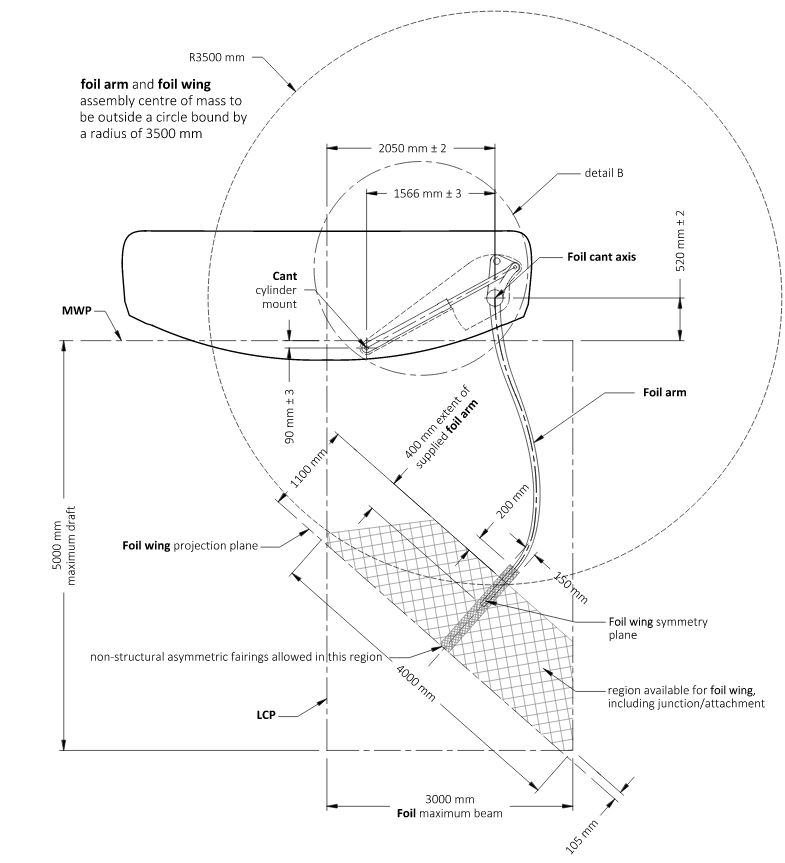
\includegraphics[height=0.8\textheight]{../../figures/AC75-class-foil.png}
\end{center}

{\footnotesize From the AC75 Class Rule}
\end{column}
\begin{column}{0.5\columnwidth}
\begin{itemize}
\item Tres grados de libertad
\begin{enumerate}
\item Àngulo de inclinación
\item Àngulo del aleron del ala
\item Àngula del aleron del timón
\end{enumerate}
\end{itemize}
\end{column}
\end{columns}
\end{frame}

\begin{frame}[label={sec:orgcea088c}]{Sistema de hidroalas - Actuadores}

\begin{center}
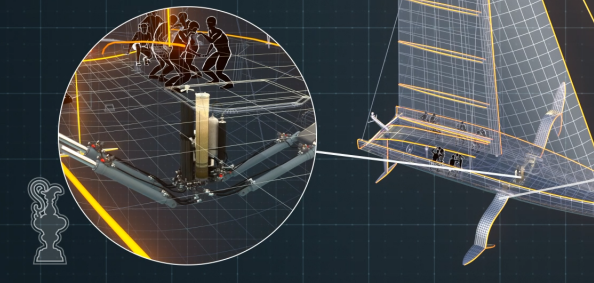
\includegraphics[height=0.4\textheight]{../../figures/AC75-actuators.png}
\end{center}

Actuadores hidraulicos con bomba electrica. Cada piston capable de producir una fuerza de 40t.
\end{frame}

\begin{frame}[label={sec:orgcf02a2f}]{Sistema de hidroalas - Señales a medir y sensores}
\begin{itemize}
\item Presión hydraulica
\item \emph{State of Charge} de las pilas
\item Posición continua de los pistones (implicando posición del ala)
\item Posición continua de los alereones
\item \emph{Yacht state}?
\end{itemize}
\end{frame}



\begin{frame}[label={sec:orgce68c92}]{Sistema de hidroalas - Control}
\begin{itemize}
\item Control en \alert{lasso cerrado}:
\begin{itemize}
\item presión hydraulica
\item posición de los pistones
\item posición de los alereones
\end{itemize}
\item Control en \alert{lasso abierto} Regla 20.1 \emph{No part of a control system may be capable of using feedback from the yacht state to control a control surface}
\end{itemize}
\end{frame}
\end{document}